%!TeX root=../tese.tex
%("dica" para o editor de texto: este arquivo é parte de um documento maior)
% para saber mais: https://tex.stackexchange.com/q/78101

\chapter{Fundamentos Teóricos}

Neste capítulo, apresentaremos os elementos teóricos que serão utilizados ao longo do desenvolvimento da pesquisa. A maior parte deste capítulo consiste em revisões de conceitos apresentados em \cite{BARRERA:04,BARRERA:03,BARRERA:02,NINA:02,DIEGO:01,NINA:01}.


%%%%%%%%%%%%%%%%%%%%%%%%%%%%%%%%%%%%%%%%%%%%%%%%%%%%%%%%%%%%%%%%%%%%%%%%%%%%%%%%%%%%
\section{Morfologia Matemática}
\label{sec:mm}

Na morfologia matemática tratamos imagens como elementos de um reticulado e transformações de imagens como operadores de reticulado. Imagens binárias com domínio $E = \mathbb{Z}^{2}$ podem ser representadas por funções do tipo $I: E \rightarrow \left\{0,1\right\}$, em que o pixel $x \in E$ da imagem $I$ é preto se, e somente se, $I(x) = 1$. Equivalentemente, uma imagem pode ser representada por um subconjunto de $E$, sendo o subconjunto $X$ gerado pela imagem com função $I$ definido como
\begin{equation*}
    X = \{x \in E: I(x) = 1\}
\end{equation*}
de forma que $X$ é formado pelos pixels preto da imagem. Os elementos de $E$ são representados por letras minúsculas como $x$, $y$ e $z$, a origem de $E$ por $o$ e os subconjuntos de E são representados por letras maiúsculas como $X$ e $S$. Daqui para frente, consideramos que uma imagem é um subconjunto $X$ de $E$.

O conjunto de todas as imagens é o conjunto potência $\mathcal{P}\left(E\right)$, também nomeado como o \textbf{conjunto das partes de um conjunto}, definido como $\mathcal{P}\left(E\right)=\left\{X:X \subseteq E\right\}$. Sendo $\subseteq$ a relação de inclusão típica de conjuntos, podemos dizer que o par $ \left( \mathcal{P}\left(E\right), \subseteq \right) $ é um \textit{conjunto parcialmente ordenado} (\textit{poset}) que possui uma estrutura de reticulado Booleano.

A seguir apresentamos algumas definições.

\begin{definition} 
        Sejam $X \in \mathcal{P}\left(E\right)$ e $z \in E$. Então, 
        $$X+z = \left\{x+z:x \in X\right\}$$
        é definido como o \textbf{translado de $X$ por $z$}. Por simplificação, também podemos denotar o transladado de $X$ por $z$ como $X_{z}$.
\end{definition}


Seja $\Psi$ a família de todos os operadores morfológicos $\psi: \mathcal{P}(E) \to \mathcal{P}(E)$ e defina em $\Psi$ a relação de ordem parcial $\psi_{1} \leq \psi_{2} \Longleftrightarrow \psi_{1} \left( X \right) \subseteq \psi_{2} \left( X \right) , \: \forall X \in \mathcal{P}\left( E \right),  \: \forall  \psi_{1},\psi_{2} \in \Psi $. O \textit{poset} $ \left( \Psi,\leq \right) $ herda a estrutura completa do reticulado $ \left( \mathcal{P}\left(E\right), \subseteq \right)$ com as seguintes definições de supremo e ínfimo.

\begin{definition} 
        O supremo e o ínfimo de um subconjunto $\Theta$ de $\Psi$ são respectivamente:
        
        $$ \left( \bigvee \Theta \right) \left( X \right) = \bigcup \left\{ \theta \left( X \right): \theta \in \Theta \right\} \ \left( X \in \mathcal{P} \left( E \right) \right) $$

        $$ \left( \bigwedge \Theta \right) \left( X \right) = \bigcap \left\{ \theta \left( X \right): \theta \in \Theta \right\} \ \left( X \in \mathcal{P} \left( E \right) \right) $$
\end{definition}



%%%%%%%%%%%%%%%%%%%%%%%%%%%%%%%%%%%%%%%%%%%%%%%%%%%%%%%%%%%%%%%%%%%%%%%%%%%%%%%%%%%%
\subsection{W-operadores}
\label{subsec:wop}

Uma classe especial de operadores morfológicos são os W-operadores, que são invariantes por translação e localmente definidos, conforme definido abaixo.

%Invariante por translação
\begin{definition} 
        Um operador $\psi: \mathcal{P}\left(E\right) \rightarrow \mathcal{P}\left(E\right)$ é dito \textbf{invariante por translação} (\textit{i.t.}) se, e somente se
        $$\psi\left(X+z\right) = \psi\left(X\right) + z \qquad \left(X \in \mathcal{P}\left(E\right), z \in E\right).$$
        \label{def:it}
\end{definition}

A invariância por translação implica que teremos um mesmo resultado se transladarmos a saída do operador por $z$ ou se transladarmos primeiro a imagem por $z$ e depois aplicarmos o operador, ou seja, a operação de translação e o operador $\psi$ comutam.

\begin{definition} 
        Seja $W \subseteq E$ um subconjunto de $E$, denominado de \textit{janela}. Um operador  $\psi: \mathcal{P}\left(E\right) \rightarrow \mathcal{P}\left(E\right)$ é \textbf{localmente definido na janela W} (\textit{l.d.}) se, e somente se
        $$x \in \psi \left(X \right) \Longleftrightarrow x \in\psi \left( X \cap \left( W+x \right) \right)$$
        para todo $x \in E$ e $X \in \mathcal{P} \left( E \right)$.
        \label{def:ld}
\end{definition}

Ou seja, um operador $\psi$ é \textit{localmente definido} em $W$ quando sua ação sobre um ponto específico do espaço depende apenas dos elementos do conjunto que estão dentro de uma vizinhança, ou "janela", ao redor desse ponto. Em outras palavras, para determinar o resultado da operação morfológica em um ponto, só é necessário analisar a configuração do conjunto dentro da janela $W$ centrada nesse ponto.

Podemos então definir, com base nos operadores \textit{i.t.} e \textit{l.d.}, os \textbf{W-operadores}.

\begin{definition} 
        Um operador $\psi_{W}: \mathcal{P}\left(E\right) \rightarrow \mathcal{P}\left(E\right)$ é denominado um \textbf{W-operador} se, e somente se ele for \textit{i.t.} e \textit{l.d.}
\end{definition}

A coleção $\Psi_{W}$ de todos os W-operadores com uma janela $W$ fixada, forma um reticulado Booleano completo e o par $ \left( \Psi_{W}, \leq \right)$ é um sub-reticulado do reticulado  $ \left( \Psi, \leq \right)$ já que é fechado por ínfimo e supremo. Ainda, cada $W$-operador é totalmente definido por uma função Booleana com domínio em $\mathcal{P}(W) \simeq \{0,1\}^{W}$, conforme o Teorema \ref{th:booleanfunction} abaixo.

\begin{theorem}
    Todo W-operador $\psi \in \Psi_{W}$, devido às propriedades de \textit{i.t.} e \textit{l.d.},  é caracterizado por uma função característica Booleana $f_{\psi}: \mathcal{P}(W) \to \{0,1\}$ definida como

    \begin{align*}
        f_{\psi} \left( X \right) = \begin{cases}
        1, & \text{se $o \in \psi \left( X \right)$},\\
        0, & \text{caso contrário}
        \end{cases} & & X \in \mathcal{P}(W),
    \end{align*}
    onde $f_{\psi}$ classifica cada ponto $\left\{0,1 \right\}^{W}$ em $\left\{0,1 \right\}$.
    \label{th:booleanfunction}
\end{theorem}

\begin{proof}
    Nós vamos mostrar que existe uma bijeção entre $\Psi_{W}$ e o conjunto de funções Booleanas de $\mathcal{P} \left( W \right)$ para $\left\{ 0,1 \right\}$. Pelas definições \ref{def:it} e \ref{def:ld} temos que, para qualquer $\psi \in \Psi_{W}, \ X \in \mathcal{P} \left( E \right) $ e $z \in E$,
    \begin{equation*}
        \begin{split}
            z \in \psi \left( X \right) \iff	z \in \psi \left( X \cap W_{z} \right) \iff z-z = o \in \left[ \psi \left( X \cap W_{z} \right) \right]_{-z} \\ \iff o \in \psi \left( \left[ X \cap W_{z} \right]_{-z} \right) \iff o \in \psi \left( X_{-z} \cap W \right)
        \end{split}
    \end{equation*}
    em que $o=\left( 0,0 \right)$ é a origem de $E$. Pelas implicações acima temos por um lado que para qualquer $f: \mathcal{P} \left( W \right) \mapsto \left\{ 0,1 \right\} $ obtemos o operador $\psi_{f} \in \Psi_{W}$ definido por
    $$z \in \psi_{h} \left( X \right) \iff f \left( X \cap W_{z} \right) = 1$$
    para qualquer $z \in E$ e $X \in \mathcal{P} \left( E \right)$. Por outro lado, de qualquer $\psi \in \Psi_{W}$ obtemos $f_{\psi} : \mathcal{P}(W) \mapsto \left\{ 0,1 \right\}$ definida como 
    \begin{equation*}
        f_{\psi} \left( X \right) = \begin{cases}
        1, & \text{se $o \in \psi \left( X \right)$},\\
        0, & \text{caso contrário}
        \end{cases},
   \end{equation*}
    para qualquer $X \in \mathcal{P} \left( W \right)$, a qual chamamos de função local ou função característica de $\psi$, estabelecendo então a bijeção. 
\end{proof} 

Além da representação pela função local $f_{\psi}$, W-operadores também podem ser representados pelo \textit{kernel} $\mathcal{K}_{W} \left( \psi \right) $ ou pela \textit{base} $\mathcal{B}_{W} \left( \psi \right) $ que serão definidos a seguir, juntamente com as definições de intervalo e intervalo maximal.

\begin{definition} 
        Seja $A, B \in \mathcal{P}\left(E\right), \ A \subseteq B $. Definimos o \textbf{intervalo fechado} com extremo esquerdo $A$ e extremo direito $B$ como       
        $$ \left[ A,B \right] = \left\{ X \in \mathcal{P}\left(E\right): A \subseteq X \subseteq B \right\}. $$        
\end{definition}

\begin{definition} 
        Seja $\textbf{X}$ uma coleção de intervalos. Chamamos $\left[A,B \right]$ de intervalo \textbf{maximal} em \textbf{X} se, e somente se,
        $$\forall \left[A',B' \right] \in \textbf{X}, \ \left[ A,B \right] \subseteq \left[A',B' \right] \Rightarrow \left[ A,B \right] = \left[ A',B' \right]. $$
        Ou seja, os intervalos maximais são aqueles que não estão contidos em nenhum outro intervalo da coleção além deles mesmos.
\end{definition}

\begin{definition} 
        Seja $\mathcal{X} \subseteq \mathcal{P}(E)$ uma coleção de subconjuntos de $E$. A coleção de todos os intervalos fechados maximais contidos em $\mathcal{X}$ é definida como,
        $$M \left( \mathcal{X} \right) = Max \left( \left\{ \left[A,B \right] \subseteq \mathcal{P}\left(E\right): \left[A,B \right] \subseteq \mathcal{X} \right\} \right)$$
\end{definition}

\begin{definition} 
        Seja $\psi_{W}$ um W-operador. O \textit{kernel} de $\psi_{W}$ é o conjunto de $\mathcal{P} \left( W \right)$ dado por
        $$\mathcal{K}_{W} \left( \psi \right) = \left\{ X \in \mathcal{P} \left( W \right): o \in \psi_{W} \left( X \right) \right\}. $$
        Equivalentemente, pelo Teorema \ref{th:booleanfunction}, o kernel pode ser definido como
        \begin{equation}
            \label{kernel_pela_fc}
            \mathcal{K}_{W} \left( \psi \right) = \left\{ X \in \mathcal{P} \left( W \right): f_{\psi}(X) = 1\right\}.
        \end{equation}
\end{definition}

\begin{definition} 
        \label{def_base}
        Seja $\psi_{W}$ um W-operador. A \textit{base} de $\psi_{W}$ como sub-coleção de $\mathcal{P} \left( W \right)$ é dada pelo conjunto de todos os intervalos maximais de $\mathcal{K}_{W} \left( \psi \right)$, ou seja, 
        $$\mathcal{B}_{W} \left( \psi \right) = M \left( \mathcal{K}_{W} \left( \psi \right)  \right) $$
\end{definition}

Qualquer W-operador pode ser representado univocamente pela base $\mathcal{B}_{W}$, pelo kernel $\mathcal{K}_{W}$ ou pela função característica $f_{\psi}$. De fato, a função característica gera o kernel pela igualdade \eqref{kernel_pela_fc} e o kernel gera a função característica pela relação
\begin{equation*}
    f_{\psi}(X) = 1 \iff X \in \mathcal{K}_{W}(\psi)
\end{equation*}
para $X \in \mathcal{P}(W)$. Ainda, o kernel gera a base pela Definição \ref{def_base} e a base gera o kernel pela igualdade
\begin{equation*}
    \mathcal{K}_{W} \left( \psi \right) =  \bigcup \{[A,B]: [A,B] \in \mathcal{B}_{W} \left( \psi \right)\}.
\end{equation*}
Logo, para realizar o aprendizado de W-operadores, é suficiente aprender seu kernel, sua base ou sua função característica. Tanto a base quanto o kernel são amplamente utilizados quando o W-operador é visto através da decomposição canônica e decomposição minimal dos mesmos. Nesse estudo será aprendida a função característica.

\textbf{****** Trazer mais detalhes sobre essas representações equivalentes ******}

\begin{figure}
  \centering
  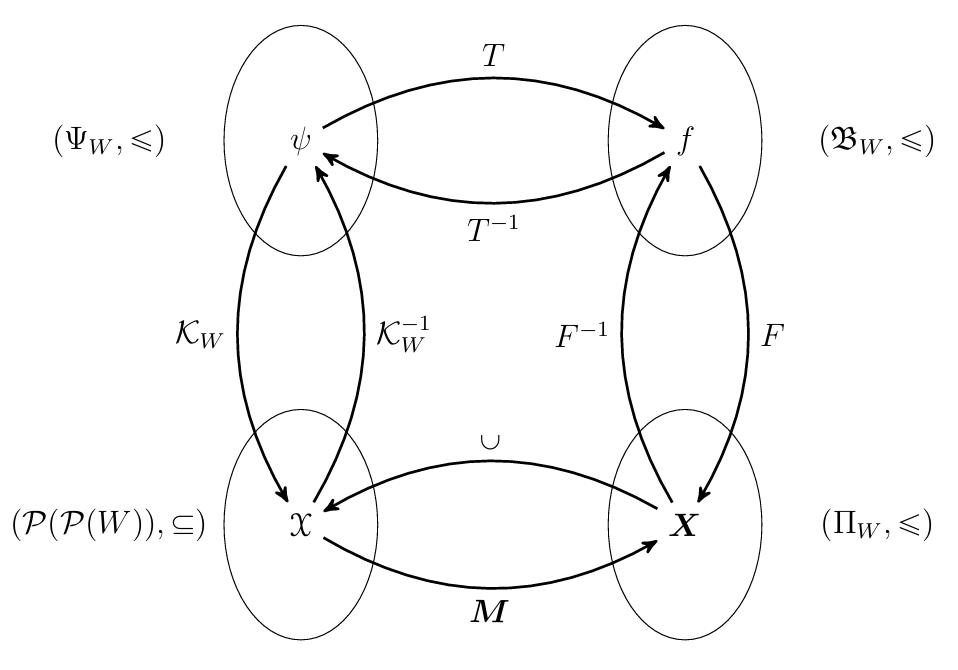
\includegraphics[width=0.75\textwidth]{figuras/lattice_isomorphism.png}
  \caption{Os isomorfismos de reticulados entre as representações dos W-operadores.\label{fig:isomorphism}}
\end{figure}

%%%%%%%%%%%%%%%%%%%%%%%%%%%%%%%%%%%%%%%%%%%%%%%%%%%%%%%%%%%%%%%%%%%%%%%%%%%%%%%%%%%%
\subsection{Projeto de W-operadores}
\label{subsec:compwop}

O projeto de W-operadores pode ser realizado por um processo de \textit{aprendizado computacional}, também conhecido como \textit{"Machine Learning"}, do tipo supervisionado, i.e., para cada exemplo observado, é fornecido também a classificação ou imagem transformada alvo do mesmo, ou seja, é dada uma coleção de pares de imagens binárias $\mathcal{S} \subseteq \mathcal{P} \left(E\right) \times \mathcal{P}\left(E\right)$, onde para todo $ \left( X,Y \right) \in \mathcal{S} $, $X$ é uma imagem que desejamos processar e $Y$ é a respectiva imagem ideal ou categoria de $X$ no caso de problemas de classificação (resultado que almejamos encontrar após o processamento de $X$). 

Esta abordagem consiste em um \textit{algoritmo de aprendizado} responsável por procurar uma função, também chamada de hipótese $h$, dentro de um espaço de hipóteses $\mathcal{H}$, i.e. $h \in \mathcal{H}$, capaz de transformar/classificar da melhor forma possível (ou com menor erro) os exemplos de treinamento. O espaço de hipóteses neste contexto é o espaço de todos os W-operadores $\Psi_{W}$ que podem ser representados pela composição de $n$ W-operadores com janelas conexas de um tamanho máximo pré-definido.

Em um processo de aprendizado buscamos sempre uma boa \textit{capacidade de generalização}. Um operador $\psi$ pode performar bem para o conjunto de imagens de treinamento $\left( X_{i},Y_{i} \right)$ (ou seja, $\psi \left( X_{i} \right) \approx Y_{i}$) e não ter uma boa generalização, performando mal para outros conjuntos de imagens $\left( X_{j},Y_{j} \right)$ (ou seja, $\psi \left( X_{j} \right) \neq Y_{j}$). Quando falamos em operador ideal ou operador ótimo em projeto de operadores, significa então encontrar um operador que tenha uma boa performance em qualquer par de imagens em um específico domínio, isto é, geradas por um mesmo processo.

Em termos estatísticos, podemos assumir que as imagens de entrada e saída são realizações de pares de conjuntos aleatórios discretos conjuntamente estacionários e cuja distribuição conjunta é caracterizada pelo W-operador com função característica $f_{\psi}: \mathcal{P} \left( W \right) \rightarrow \left\{ 0,1 \right\}$. Podemos considerar então que o processo local $S_{z} = X_{-z} \cap W = \left( X \cap W_{z} \right)_{-z} $ e $i_{z} = Y \left( z \right), z \in E, $ segue uma distribuição de probabilidade $P \left( S_{z}, \ i_{z} \right)$ fixada, mas desconhecida.

O operador $\psi$ é considerando um estimador de $Y$ com um erro de estimação definido em termos de uma função de perda $\ell: \psi \left( X \right) \times Y \to \mathbb{R}_{\geq0} $. O operador ótimo será aquele com menor erro dado pela perda esperada em qualquer posição $z$ por $R_{\ell} \langle \psi \rangle =  E_{P} \left[ \ell \left( f_{\psi} \left( S_{z} \right),i_{z} \right) \right]$, em que a esperança é em relação à distribuição $P$ que gerou os dados. Por exemplo, se a função de perda é a diferença absoluta $\ell \left(a,b \right)= \left| a-b \right|$ o erro esperado é o \textbf{MAE} - \textit{erro esperado médio} - em que fixada uma posição $z$, $MAE \langle \psi \rangle =E_{P} \left[ | f_{\psi} \left( S_{z} \right) - i_{z} | \right]$.

\begin{definition} 
        Dizemos que $\psi^{*} \in \Psi_{W} $ é ótimo em $\Psi_{W}$, segundo a função de perda $\ell$ se, e somente se  $R_{\ell} \langle \psi^{*} \rangle \leq R_{\ell} \langle \psi \rangle$, para todo $\psi \in \Psi_{W} $.
\end{definition}

Chamamos $R_{\ell} \langle \psi \rangle$ de \textit{out-of-sample error}, uma vez que o erro esperado é sob a distribuição $P$ que gerou os dados. Como $P$ é desconhecida, calculamos o erro empírico sob uma amostra de treinamento $\mathcal{D}_{N_{t}}$, onde $\mathcal{D}_{N_{t}} = \left\{ \left( X_{i}, Y_{i} \right) \ : \ 1 \leq i \leq N_{t} \right\}$ são $N_{t}$ pares $(X,Y)$ de imagens de entrada e de saída. Para cada operador $\psi \in \Psi_{W}$ definimos $L_{t}(\psi)$ como o seu erro empírico, ou \textit{in-sample-error}, que é a média amostral de $\sum\limits_{z} \ell \left( f_{\psi} \left( S_{z} \right),i_{z} \right)$.

É possível também incluir uma regularização implícita no processo de aprendizado através de uma amostra de validação $\mathcal{D}_{M}^{(val)}$, em que a amostra de treinamento é dividida de forma prévia e aleatória em duas, tal que, fixado um $M + N = N_{t}$ e , temos
$$\mathcal{D}_{N}^{(train)} = \left\{ (X_{i},Y_{i}): 1 \leq i \leq N \right\}$$
$$\mathcal{D}_{M}^{(val)} = \left\{ (X_{i},Y_{i}): N < i \leq N + M \right\}$$
Por simplificação, chamaremos a partir deste ponto $\mathcal{D}_{N}^{(train)}$ de $\mathcal{D}_{N}$ e $\mathcal{D}_{M}^{(val)}$ de $\tilde{\mathcal{D}}_{M}$, cujos erros empíricos (in-sample) denotamos por $L_{t}$ e $L_{v}$, respectivamente.

As instâncias na amostra de validação não estão nos dados de treinamento e assim fornecem informações com menor viés sobre a qualidade de generalização da hipótese selecionada. Assim realizaremos o aprendizado baseando-se nos dois erros $L_{t}$ e $L_{v}$.


%%%%%%%%%%%%%%%%%%%%%%%%%%%%%%%%%%%%%%%%%%%%%%%%%%%%%%%%%%%%%%%%%%%%%%%%%%%%%%%%%%%%
\subsection{Composição de W-operadores}
\label{subsec:compwop}

É possível obter um operador pela composição de operadores mais simples. Quando em um problema é necessário extrair diversas \textit{features} da imagem, como ruídos, filtragem de arestas ou segmentação de objetos, cada operador simples pode focar em um desses subproblemas e o operador final, que resolve o problema como um todo, é obtido pela composição sequencial desses operadores iniciais. 

Formalmente, seja $\theta = \left\{ \psi_{1}, ..., \psi_{n} \right\}, \ n \geq 2$, uma sequência de $n$ W-operadores com janelas $W_{1}, ...,  W_{n} $ e funções características $f_{1}, ..., f_{n}$. Definimos o W-operador multicamadas dado pela composição dos $n$ operadores em $\theta$ como
$$ \psi_{\theta} = \psi_{n} \circ \cdot \cdot \cdot \circ \psi_{1}. $$
O operador $\psi_{\theta}$ é \textit{i.t.} e \textit{l.d.} dentro da janela
$$W_{\theta} = W_{1} \oplus \cdot \cdot \cdot \oplus W_{n} $$
que seria a soma de Minkowski das $n$ janelas. 

Supondo que um operador $ \psi_{\theta} $ realize $n$ iterações sobre uma mesma janela $W$, temos então $n \times 2^{ \left| W \right|}$ parâmetros que precisam ser estimados, que são a imagem da função característica de cada operador. Já para um operador composto $\psi$ com janela $W^{\prime} = W_{1} \oplus \cdots \oplus W_{n}$, sendo $W_{i} = W$ para qualquer $i=1,...,n$, temos $2^{\left| W^{\prime} \right|}$ parâmetros. Por exemplo, se $W = W_{3 \times 3}$, $n = 2$ e $W^{\prime} = W \oplus W$, então $W^{\prime} = W^{\prime}_{5 \times 5}$ e para projetar o operador de 2 iterações sobre $W^{\prime}$ precisamos de $2 \times 2^{9} = 2^{10}$ parâmetros, enquanto para projetar diretamente o operador $\psi$ precisamos estimar $2^{25}$ parâmetros. Assim sendo, vemos que projetar um operador de forma composta possui muito menos parâmetros, o que indica que a sua precisão pode ser muito melhor que a precisão se projetássemos diretamente o operador final.

%%%%%%%%%%%%%%%%%%%%%%%%%%%%%%%%%%%%%%%%%%%%%%%%%%%%%%%%%%%%%%%%%%%%%%%%%%%%%%%%%%%%
\section{Espaço de Aprendizado}
\label{sec:ls}

O espaço de hipóteses $\mathcal{H}$ é um conjunto de hipóteses, que neste contexto serão W-operadores multicamadas. Um espaço $\mathcal{H}$ pode ser decomposto em sub-conjuntos chamados de modelos $\{\mathcal{M}_{1},\dots,\mathcal{M}_{k}\}, \mathcal{M}_{i} \subseteq \mathcal{H},$ de forma que
$$\mathcal{H} = \bigcup_{i=i}^{k} \mathcal{M}_{i}, $$
e uma possível abordagem de aprendizado nesse contexto seria primeiro selecionar um modelo dentre os candidatos, e então aprender uma hipótese nesse modelo.

Algoritmos tradicionais de \textit{seleção de modelos} buscam de forma exaustiva o melhor modelo baseado nos dados, primeiro encontrando a melhor hipótese em cada modelo, minimizando o erro em uma amostra de treinamento, e selecionando o modelo cuja hipótese encontrada minimiza o erro em uma amostra de validação.

Um Espaço de Aprendizado $\mathbb{L} \left( \mathcal{H} \right)$, também conhecido como \textit{Learning Space} (LS), é uma família de modelos candidatos parcialmente ordenados por inclusão, ou seja, um \textit{poset} de subespaços de $\mathcal{H}$, que pode ser projetada com conhecimento a priori e restrições específicas para cada classe de problemas. Além disso, alguns LS possuem uma estrutura com propriedades que podem ser aproveitadas na implementação de algoritmos não exaustivos de \textit{seleção de modelos} que, quando aliadados a alto poder computacional, permitem resolver problemas práticos que requerem algoritmos de alta complexidade \cite{DIEGO:01}. Abaixo definimos o LS. A dimensão VC de um espaço de hipóteses é uma medida da sua complexidade, cuja definição formal pode ser encontrada em \cite{DIEGO:01}.

\begin{definition} 
        Seja $\ell$ uma função de perda fixada e $\mathcal{H}$ um espaço de hipótese genérico com dimensão VC finita, $d_{VC} \left( \mathcal{H},\ell \right) < \infty	$. Seja $\mathbb{L} \left( \mathcal{H} \right):= \left\{ \mathcal{M}_{i} \ : \ i \in \mathcal{J} \subseteq \mathbb{Z}_{+}  \right\} $ um subconjunto finito do conjunto potência de $\mathcal{H}$, ou seja, $\mathbb{L} \left( \mathcal{H} \right) \subseteq \mathcal{P} \left( \mathcal{H} \right)$ e $ \left| \mathcal{J} \right| < \infty$. Dizemos que o \textit{poset} $ \left( \mathbb{L} \left( \mathcal{H} \right), \subseteq  \right)$ é um \textbf{Espaço de Aprendizado} sob a função de perda $\ell$ se,
        
        $ \left( i \right) \: \bigcup_{i \in \mathcal{J}} \mathcal{M}_{i} = \mathcal{H}$;
        
        $ \left( ii \right) \: \mathcal{M}_{1} , \mathcal{M}_{2} \in \mathbb{L} \left( \mathcal{H} \right) $ e $  \mathcal{M}_{1} \subseteq  \mathcal{M}_{2}$ implica em $d_{VC} \left( \mathcal{M}_{1},\ell \right) < d_{VC} \left( \mathcal{M}_{2},\ell \right) $

        Definimos a dimensão VC de $ \mathbb{L} \left( \mathcal{H} \right)$ como
        $$d_{VC} \left( \mathbb{L} \left( \mathcal{H} \right),\ell \right) := \max_{i \in \mathcal{J}}d_{VC} \left( \mathcal{M}_{i},\ell \right) $$
        cujo limite superior é $d_{VC} \left( \mathcal{H},\ell \right)$.
        \label{def:ls}
\end{definition}

Como $\mathbb{L} \left( \mathcal{H} \right)$ cobre $ \mathcal{H} $, quando buscamos um modelo em $\mathbb{L} \left( \mathcal{H} \right)$, nenhuma hipótese será descartada de antemão, mas uma restrição em $\mathcal{H}$ poderá ser aplicada somente a \textit{posteriori} e baseada nos dados.

Existem múltiplos subconjuntos de $\mathcal{P} \left( \mathcal{H} \right)$ que são LS, porém alguns subconjuntos, chamados de \textit{Lattice Learning Spaces}, possuem as propriedades de reticulado, que propiciam uma melhor eficiência nos algoritmos de seleção de modelo. O LS considerado neste trabalho faz parte dessa classe.

\begin{definition}
    Seja $\mathbb{L} \left( \mathcal{H} \right)$ um LS de $\mathcal{H}$. $\mathbb{L} \left( \mathcal{H} \right)$ será um \textbf{Lattice Learning Space} se $\left( \mathbb{L} \left( \mathcal{H} \right), \subseteq,\wedge,\vee, \mathcal{O}, \mathcal{I} \right)$ for um reticulado completo, que é um \textit{poset} com o menor $\left( \mathcal{O} \right)$ e maior $\left( \mathcal{I} \right)$ modelo, e com os operadores supremo $\vee$ e ínfimo $\wedge$ definidos para todos os subconjuntos de $\mathbb{L} \left( \mathcal{H} \right)$.
\end{definition}

\subsection{Cadeias Contínuas}

\textit{Cadeias Contínuas} no LS são cadeias sem saltos nos modelos em $\mathbb{L} \left( \mathcal{H} \right)$ quando consideramos a distância direta no grafo acíclico correspondente ao $\left( \mathbb{L} \left( \mathcal{H} \right),\subseteq \right)$, denotada por $d \left( \cdot , \cdot \right)$, conforme exemplificado na Figura \ref{fig:cadeia}.

\begin{definition}
    Uma sequência $\mathcal{M}_{i_{1}} \subseteq \mathcal{M}_{i_{2}} \subseteq \cdot \cdot \cdot \subseteq \mathcal{M}_{i_{k}} $ é chamada de \textbf{cadeia contínua} de $\mathbb{L} \left( \mathcal{H} \right)$ se, e somente se,
    $$d \left( \mathcal{M}_{i_{j}},\mathcal{M}_{i_{j+1}} \right) = 1 \; \text{para todo } j \in \left\{ 1,...,k-1 \right\}$$ 
\end{definition}

\begin{figure}
  \centering
  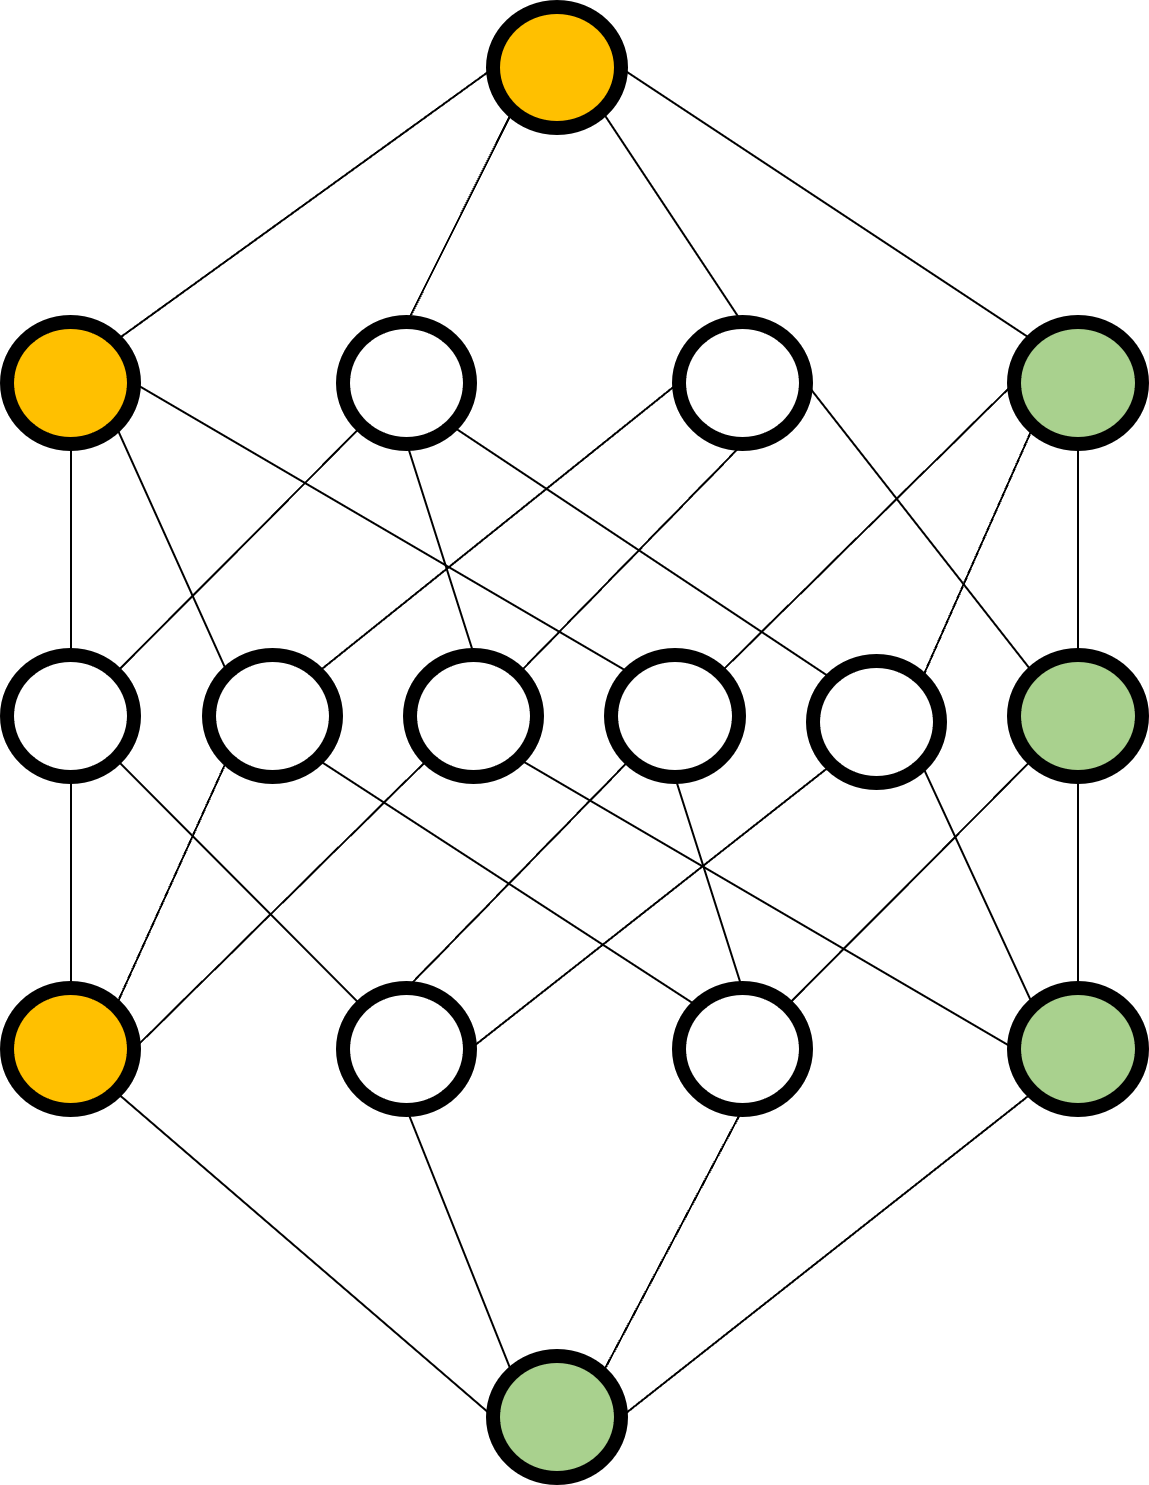
\includegraphics[width=.4\textwidth]{figuras/cadeia.png}
  \caption{Exemplo de uma cadeia contínua (verde) e uma cadeia não contínua (amarelo) em um LS Booleano.\label{fig:cadeia}}
\end{figure}

\subsection{Mínimos no Espaço de Aprendizado}

Seleção de modelos via LS depende do conceito de \textit{mínimos} de um $\mathbb{L} \left( \mathcal{H} \right)$ quando o erro de um modelo $\mathcal{M}$ é estimado por um estimador fixo $\hat{L} \left( \mathcal{M} \right)$.

\begin{definition}
    O modelo $\mathcal{M}_{i_{j^{*}}}$ é,
    \begin{itemize}
        \item Um \textbf{mínimo local fraco} de uma cadeia contínua  $\mathcal{M}_{i_{1}} \subseteq \mathcal{M}_{i_{2}} \subseteq \cdot \cdot \cdot \subseteq \mathcal{M}_{i_{k}} $ de $\mathbb{L} \left( \mathcal{H} \right)$ se
        $$\hat{L} \left( \mathcal{M}_{i_{j^{*}}} \right) \leq \min \left( \hat{L} \left( \mathcal{M}_{i_{j^{*}-1}} \right), \hat{L} \left( \mathcal{M}_{i_{j^{*}+1}} \right)  \right)$$
        onde $\hat{L} \left( \mathcal{M}_{i_{0}} \right) \equiv \hat{L} \left( \mathcal{M}_{i_{k+1}} \right) \equiv + \infty  $ ;

        \item Um \textbf{mínimo local forte} de $\mathbb{L} \left( \mathcal{H} \right)$ é um mínimo local fraco de todas as cadeias contínuas de $\mathbb{L} \left( \mathcal{H} \right)$ que o contém, ou seja,
        $$\hat{L} \left( \mathcal{M}_{i_{j^{*}}} \right) \leq \min \left\{ \hat{L} \left( \mathcal{M} \right) \ : \ \mathcal{M} \in \mathbb{L} \left( \mathcal{H} \right), \ d \left( \mathcal{M}_{i_{j^{*}}}, \mathcal{M} \right) = 1 \right\} \text{;}$$

        \item Um \textbf{sup-mínimo local fraco} de $\mathbb{L} \left( \mathcal{H} \right)$ se,
        $$\hat{L} \left( \mathcal{M}_{i_{j^{*}}} \right) \leq \min \left\{ \hat{L} \left( \mathcal{M} \right) \ : \ \mathcal{M} \in \mathbb{L} \left( \mathcal{H} \right), \ \mathcal{M}_{i_{j^{*}}} \subseteq \mathcal{M} \ ,\ d \left( \mathcal{M}_{i_{j^{*}}}, \mathcal{M} \right) = 1 \right\} \text{;}$$

        \item Um \textbf{inf-mínimo local fraco} de $\mathbb{L} \left( \mathcal{H} \right)$ se,
        $$\hat{L} \left( \mathcal{M}_{i_{j^{*}}} \right) \leq \min \left\{ \hat{L} \left( \mathcal{M} \right) \ : \ \mathcal{M} \in \mathbb{L} \left( \mathcal{H} \right), \ \mathcal{M} \subseteq \mathcal{M}_{i_{j^{*}}} \ ,\ d \left( \mathcal{M}_{i_{j^{*}}}, \mathcal{M} \right) = 1 \right\} \text{;}$$

        \item Um \textbf{mínimo global} de uma cadeia contínua se,
        $$ \hat{L}  \left( \mathcal{M}_{i_{j^{*}}} \right) = \min_{1 \leq j \leq k} \hat{L}  \left( \mathcal{M}_{i_{j}} \right) \text{;}$$

        \item Um \textbf{mínimo global} de $\mathbb{L} \left( \mathcal{H} \right)$ se,
        $$ \hat{L}  \left( \mathcal{M}_{i_{j^{*}}} \right) = \min_{1 \in \mathcal{J}} \hat{L}  \left( \mathcal{M}_{i_{j}} \right) \text{.}$$
        
    \end{itemize}
    \label{def:minimos}
\end{definition}

\subsection{O Aprendizado de Hipóteses via Espaço de Aprendizado}

O \textit{framework} de LS para aprender hipóteses é composto de dois passos:

\begin{enumerate}
    \item Aprender um modelo $\hat{\mathcal{M}}$ em $\mathbb{L} \left( \mathcal{H} \right)$ pela minimização da medida de erro $\hat{L}$. Formalmente, sendo    
    $$\hat{\mathcal{L}} =  \underset{\mathcal{M}\in \mathbb{L}\left( \mathcal{H}\right)}{\arg \min} \  \hat{L} \left( \mathcal{M} \right)$$
    os modelos que minimizam $\hat{L}$ em $\mathbb{L}(\mathcal{H})$, aprendemos   
   $$\hat{\mathcal{M}} =  \underset{\mathcal{M}\in \hat{\mathcal{L}}}{\arg \min} \  d_{VC} \left( \mathcal{M} \right)$$
   que é o modelo mais simples dentre os mínimos globais.

   \item Aprender uma hipótese em $\hat{\mathcal{M}}$ pela minimização do erro empírico $L_{t}$ em uma amostra $\mathcal{D}_{N}$. Formalmente, a hipótese aprendida será
   $$ \hat{h}_{\hat{\mathcal{M}}}^{\mathcal{D}_{N}} := \underset{h \in \hat{\mathcal{M}}}{\arg \min} \ L_{D_{N}} \left( h \right)$$
\end{enumerate}


%%%%%%%%%%%%%%%%%%%%%%%%%%%%%%%%%%%%%%%%%%%%%%%%%%%%
\section{U-curve no Espaço de Aprendizado}
\label{sec:ucurve}

Quando modelos são organizados em estruturas de reticulado, apesar de frequentemente não termos a prova matemática, temos evidências empíricas do comportamento heurístico de propriedade de U-curve no LS. As propriedades U-curve são uma das poucas que garantem rigorosamente uma solução ótima sem a necessidade de uma busca exaustiva de todos os modelos candidatos no espaço de aprendizado. Mesmo quando a propriedade não é totalmente satisfeita, ou comprovada, é possível utilizar-se dela e encontrar uma solução sub-ótima aceitável.

Um exemplo do fenômeno de U-curve se dá conforme caminhamos em uma cadeia de modelos $\mathcal{M}_{0} \subseteq \cdot \cdot \cdot \subseteq \mathcal{M}_{6}$ onde a complexidade (em termos de dimensão VC) vai aumentando, sendo $\mathcal{M}_{0}$ menos complexo e $\mathcal{M}_{6}$ mais complexo. A princípio o erro estimado $\hat{L}$ diminui até encontrar um ponto de inflexão e começar a monotonicamente crescer com o aumento da complexidade, conforme ilustrado na Figura \ref{fig:ucurve}. Este fenômeno, quando atrelado ao aumento do número de variáveis e/ou parâmetros dos modelos, é conhecido como fenômeno de pico (\textit{peaking phenomenon}), conforme ilustrado em \cite{ucurve:06,ucurve:01, ucurve:02, ucurve:03, ucurve:05, ucurve:04}.

\begin{figure}
  \centering
  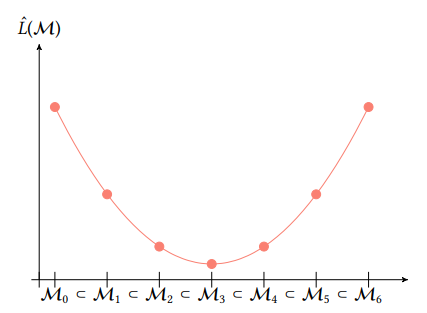
\includegraphics[width=.4\textwidth]{figuras/u_curve.png}
  \caption{Ilustração do fenômeno de U-curve apresentada por \cite{DIEGO:01} em uma cadeia de modelos com aumento de complexidade.\label{fig:ucurve}}
\end{figure}

 
 %\subsection{Propriedades de U-curve}
 Podemos definir as \textbf{Propriedades de U-curve} baseando-se nas Definições em \ref{def:minimos} e no estimador $\hat{L}$.

 \begin{definition}
     Um LS $\mathbb{L} \left( \mathcal{H} \right)$ sob uma função de perda $\ell$ e um estimador $\hat{L}$ satisfaz:

     \begin{itemize}
         \item \textbf{Propriedade U-curve Forte} se todos os mínimos locais fracos de uma cadeia contínua de $\mathbb{L} \left( \mathcal{H} \right)$ são um mínimo global dessa cadeia;

         \item \textbf{Propriedade U-curve Fraca} se todos os mínimos locais fortes são um mínimo global de todas as cadeias contínuas de $\mathbb{L} \left( \mathcal{H} \right)$ que o contém;

         \item \textbf{Propriedade U-curve Sup-Fraca} se todos os sup-mínimos locais fortes possuem um erro estimado menor ou igual ao de todos os modelos em $\mathbb{L} \left( \mathcal{H} \right)$ que o contém;

         \item \textbf{Propriedade U-curve Inf-Fraca} se todos os inf-mínimos locais fortes possuem um erro estimado menor ou igual ao de todos os modelos em $\mathbb{L} \left( \mathcal{H} \right)$ que o contém;
     \end{itemize}

     As condições que caracterizam as propriedades de U-curve devem ser verdade com probabilidade 1, válida para todas as possíveis amostras sob as quais $\hat{L}$ é calculada.
 \end{definition}


Podemos aproveitar as propriedades U-curve em um algoritmo de minimização de $\hat{L}$ para evitar uma busca exaustiva de $\mathbb{L} \left( \mathcal{H} \right)$. 
 
Caso a propriedade U-curve Forte seja satisfeita, o Algoritmo U-curve deve percorrer todas as cadeias contínuas de $\mathbb{L} \left( \mathcal{H} \right) $ até encontrar o seu (único) mínimo local fraco, de modo que encontremos todos os mínimos locais fracos e, portanto, o mínimo global. Similarmente, caso a propriedade U-curve Fraca seja satisfeita, o Algoritmo U-curve deve percorrer todas as cadeias contínuas de $\mathbb{L} \left( \mathcal{H} \right) $ até encontrar o seu (único) mínimo local forte, de modo que encontremos todos os mínimos locais fortes e, portanto, o mínimo global. Nos dois cenários, $\mathbb{L} \left( \mathcal{H} \right) $ não é percorrido exaustivamente, pois uma vez que encontramos um mínimo local forte ou fraco não precisamos calcular o erro dos modelos restantes da cadeia.

Por outro lado, se a propriedade U-curve Sup-Fraca (ou Inf-Fraca) for satisfeita, podemos percorrer todas as cadeias contínuas de $\mathbb{L} \left( \mathcal{H} \right) $ até encontrarmos um sup-mínimo (inf-mínimo) local forte e, portanto, o mínimo global. Neste caso $\mathbb{L} \left( \mathcal{H} \right) $ também não é percorrido exaustivamente, pois quando encontramos um sup-mínimo (inf-mínimo) local forte não precisamos calcular o erro dos modelos maiores (menores) da cadeia contínua.

Por fim, quando as propriedades U-curve não são estritamente satisfeitas e ainda assim utilizarmos o Algoritmo U-curve, teremos uma solução sub-ótima, uma vez que podemos perder o mínimo global quando não visitamos o restante dos modelos da cadeia ao encontrar o seu respectivo mínimo local. Ainda assim o algoritmo pode retornar um mínimo local com baixo erro e ser suficiente para a aplicação prática em questão.